\documentclass[
	10pt,								% globale Schriftgröße
	parskip=half-,						% setzt Absatzabstand hoch
	paper=a4,							% Format
	english,ngerman,					% lädt Sprachpakete
	]{scrartcl}							% Dokumentenklasse

% //////////////////// Pakete laden ////////////////////
\usepackage{amsmath}			% MUSS vor fontspec geladen werden
\usepackage{mathtools}			% modifiziert amsmath
\usepackage{amssymb}			% mathematische symbole, für \ceckmarks
\usepackage{amsthm}				% für proof
\usepackage{mathrsfs}			% für \mathscr
\usepackage{latexsym}
\usepackage{marvosym}				% für Lightning

\usepackage{fontspec} 			% funktioniert nur mit den neueren Compilern z.B. XeLaTeX
\usepackage{microtype}			% für bessere Worttrennung
\usepackage[ngerman]{babel} 	% Spracheinstellung
\usepackage{lmodern}			% verändert verwendete Schriftart, damit sie weniger pixelig ist

\usepackage{verbatim}
\usepackage{listings}			% Für Quellcode

\usepackage{graphicx}
\usepackage{tabularx}			% für Tabellen mit gleicher Spaltenbreite und automatischen Umbrüchen
\usepackage{fullpage}
\usepackage{multirow}			% für multirow in tabulars
\usepackage{rotate}
\usepackage[cmyk,table]{xcolor} % um Farben zu benutzen, kann mehr als das Paket color
\usepackage[					% Verlinkungen
	colorlinks,					% farbige Schrift, statt farbiger Rahmen
	linktocpage,				% verlinkt im Abb.Verzeichnis Seitenzahl statt Bildunterschrift
	linkcolor=blue				% setzt Farbe der Links auf blau
	]{hyperref}					% nur für digitale Anwendungen, url = "http://www.example.com"
\usepackage{url}				% für Webadressen wie e-mail usw.: "\url{http://www.example.com}"

\usepackage{enumerate}			% für versch. Aufzählungezeichen wie z.B. a)
\usepackage{xspace}				% folgt ein Leerzeichen nach einem \Befehl, wird es nicht verschluckt.
\usepackage{cancel}				% für das Durchstreichen u.a. in Matheformeln mit \cancel
\usepackage{float}              % zum Forcieren der Position von figure-Umgebungen

% zum Zeichnen (u.a. von Graphen)
\usepackage{fp}
\usepackage{tikz}
\usetikzlibrary{tikzmark}			% für \tikzmark{toRemember}
\usetikzlibrary{positioning}	% verbesserte Positionierung der Knoten
\usetikzlibrary{automata}		% für Automaten (GTI)
\usetikzlibrary{arrows}
\usetikzlibrary{shapes}
\usetikzlibrary{decorations.pathmorphing}
\usetikzlibrary{decorations.pathreplacing}
\usetikzlibrary{decorations.shapes}
\usetikzlibrary{decorations.text}

% //////////////////// Syntaxhighlighting ////////////////////
\lstloadlanguages{Python, Haskell, [LaTeX]TeX, Java}
\lstset{
   basicstyle=\footnotesize\ttfamily,	% \scriptsize the size of the fonts that are used for the code
   backgroundcolor = \color{bgcolour},	% legt Farbe der Box fest
   breakatwhitespace=false,	% sets if automatic breaks should only happen at whitespace
   breaklines=true,			% sets automatic line breaking
   captionpos=t,				% sets the caption-position to bottom, t for top
   commentstyle=\color{codeblue}\ttfamily,% comment style
   frame=single,				% adds a frame around the code
   keepspaces=true,			% keeps spaces in text, useful for keeping indentation
							% of code (possibly needs columns=flexible)
   keywordstyle=\bfseries\ttfamily\color{codepurple},% keyword style
   numbers=left,				% where to put the line-numbers;
   							% possible values are (none, left, right)
   numberstyle=\tiny\color{codegreen},	% the style that is used for the line-numbers
   numbersep=5pt,			% how far the line-numbers are from the code
   stepnumber=1,				% nummeriert nur jede i-te Zeile
   showspaces=false,			% show spaces everywhere adding particular underscores;
							% it overrides 'showstringspaces'
   showstringspaces=false,	% underline spaces within strings only
   showtabs=false,			% show tabs within strings adding particular underscores
   flexiblecolumns=false,
   tabsize=1,				% the step between two line-numbers. If 1: each line will be numbered
   stringstyle=\color{orange}\ttfamily,	% string literal style
   numberblanklines=false,				% leere Zeilen werden nicht mitnummeriert
   xleftmargin=1.2em,					% Abstand zum linken Layoutrand
   xrightmargin=0.4em,					% Abstand zum rechten Layoutrand
   aboveskip=2ex, 
}

\lstdefinestyle{py}{
   language=Python,
}
\lstdefinestyle{hs}{
   language=Haskell,
}
\lstdefinestyle{tex}{
	language=[LaTeX]TeX,
	escapeinside={\%*}{*)},     % if you want to add LaTeX within your code
	texcsstyle=*\bfseries\color{blue},% hervorhebung der tex-Schlüsselwörter
	morekeywords={*,$,\{,\},\[,\],lstinputlisting,includegraphics,
	rowcolor,columncolor,listoffigures,lstlistoflistings,
	subsection,subsubsection,textcolor,tableofcontents,colorbox,
	fcolorbox,definecolor,cellcolor,url,linktocpage,subtitle,
	subject,maketitle,usetikzlibrary,node,path,addbibresource,
	printbibliography},% if you want to add more keywords to the set
     numbers=none,
     numbersep=0pt,
     xleftmargin=0.4em,
}

\lstdefinestyle{java}{
	language=Java,
	extendedchars=true,		% lets you use non-ASCII characters;
   						% for 8-bits encodings only, does not work with UTF-8
}

\lstdefinelanguage[x64]{Assembler}     % add a "x64" dialect of Assembler
   [x86masm]{Assembler} % based on the "x86masm" dialect
   % with these extra keywords:
   {morekeywords={CDQE,CQO,CMPSQ,CMPXCHG16B,JRCXZ,LODSQ,MOVSXD, %
                  POPFQ,PUSHFQ,SCASQ,STOSQ,IRETQ,RDTSCP,SWAPGS, %
                  rax,rdx,rcx,rbx,rsi,rdi,rsp,rbp, %
                  r8,r8d,r8w,r8b,r9,r9d,r9w,r9b}
}					% for 8-bits encodings only, does not work with UTF-8

\lstdefinestyle{c}{
	language=c,
	extendedchars=true,		% for 8-bits encodings only, does not work with UTF-8
}

% //////////////////// eigene Kommandos ////////////////////
\newcommand\FU{Freie Universität Berlin\xspace}% benötigt package xspace
\newcommand\gdw{g.\,d.\,w.\xspace}
\newcommand\oBdA{o.\,B.\,d.\,A.\xspace}
\newcommand{\Eu}{\texteuro}
\newcommand\N{\mathbb{N}\xspace}
\newcommand\Q{\mathbb{Q}\xspace}
\newcommand\R{\mathbb{R}\xspace}
\newcommand\Z{\mathbb{Z}\xspace}
\newcommand\ohneNull{\ensuremath{\backslash\lbrace 0\rbrace}}% \{0}
\let\dhALT\dh	% Schreibt Befehl \dh in \dhALT um
\renewcommand\dh{d.\,h.\xspace}	%renew überschreibt command \dh
\newcommand\Bolt{\;\text{\LARGE\raisebox{-0.3em}{\Lightning}\normalsize}\xspace}% Blitz
\newcommand\zz{\ensuremath{\raisebox{+0.25ex}{Z}% zu zeigen
			\kern-0.4em\raisebox{-0.25ex}{Z}%
			\;\xspace}}
\newcommand{\from}{\ensuremath{\colon}}
\newcommand{\floor}[1]{\lfloor{#1}\rfloor}
\newcommand{\ceil}[1]{\lceil{#1}\rceil}
 \renewcommand{\L}{\ensuremath{\mathcal{L}}\xspace}
 \renewcommand{\P}{\ensuremath{\mathcal{P}}\xspace}
 \newcommand{\NL}{\ensuremath{\mathcal{N}\kern-0.2em\mathcal{L}}\xspace}
 \newcommand{\NP}{\ensuremath{\mathcal{NP}}\xspace}

% //////////////////// Mathefunktionen ////////////////////
\DeclareMathOperator{\Landau}{\mathcal{O}}
\DeclareMathOperator{\True}{True}
\DeclareMathOperator{\False}{False}

% //////////////////// eigene Theoreme ////////////////////
\newtheorem{theorem}{Satz}
\newtheorem{corollary}[theorem]{Folgerung}
\newtheorem{lemma}[theorem]{Lemma}
\newtheorem{observation}[theorem]{Beobachtung}
\newtheorem{definition}[theorem]{Definition}
\newtheorem{Literatur}[theorem]{Literatur}
% konfiguriert proof
\makeatletter
\newenvironment{Proof}[1][\proofname]{\par
  \pushQED{\qed}%
  \normalfont \topsep6\p@\@plus6\p@\relax
  \trivlist
  \item[\hskip\labelsep
%         \itshape
        \bfseries
    #1\@addpunct{.}]\ignorespaces
}{%
  \popQED\endtrivlist\@endpefalse
}
\makeatother

% //////////////////// eigene Farben ////////////////////
\let\definecolor=\xdefinecolor
\definecolor{FUgreen}{RGB}{153,204,0}
\definecolor{FUblue}{RGB}{0,51,102}

\definecolor{middlegray}{rgb}{0.5,0.5,0.5}
\definecolor{lightgray}{rgb}{0.8,0.8,0.8}
\definecolor{orange}{rgb}{0.8,0.3,0.3}
\definecolor{azur}{rgb}{0,0.7,1}
\definecolor{yac}{rgb}{0.6,0.6,0.1}
\definecolor{Pink}{rgb}{1,0,0.6}

\definecolor{bgcolour}{rgb}{0.97,0.97,0.97}
\definecolor{codegreen}{rgb}{0,0.6,0}
\definecolor{codegray}{rgb}{0.35,0.35,0.35}
\definecolor{codepurple}{rgb}{0.58,0,0.82}
\definecolor{codeblue}{rgb}{0.4,0.5,1}

% //////////////////// eigene Settings ////////////////////

\textheight = 230mm		% Höhe des Satzspiegels / Layouts
\footskip = 10ex			% Abstand zw. Fußzeile und Grundlinie letzter Textzeile
\parindent 0pt			% verhindert Einrückung der 1. Zeile eines Absatzes
\setkomafont{sectioning}{\rmfamily\bfseries}% setzt Ü-Schriften in Serifen, {disposition}

\newcommand{\dozent}{Lutz Prechelt}
\newcommand{\tutor}{Samuel Domiks}
\newcommand{\tutoriumNo}{02\\Materialien: Latex, Skript}
\newcommand{\ubungNo}{12}
\newcommand{\veranstaltung}{Softwaretechnik}
\newcommand{\semester}{SoSe21}
\newcommand{\studenten}{Jonny Lam \& Thore Brehmer}

% /////////////////////// BEGIN DOKUMENT /////////////////////////
\begin{document}
% /////////////////////// BEGIN TITLEPAGE /////////////////////////
\begin{titlepage}
	\subject{\dozent}
	\title{\veranstaltung, \semester}
	\subtitle{\Large Übung \ubungNo\\ \large\vspace{1ex} TutorIn: \tutor\\ Tutorium \tutoriumNo}
	\author{\studenten}
	\date{\normalsize \today}
\end{titlepage}

\maketitle								% Erstellt das Titelblatt
\vspace*{-10cm}							% rückt Logo an den oberen Seitenrand
\makebox[\dimexpr\textwidth+1cm][r]{	%rechtsbündig und geht rechts 1cm über Layout hinaus
	
\includegraphics[width=0.4\textwidth]{src/fu_logo} % fügt FU-Logo ein
}
% /////////////////////// END TITLEPAGE /////////////////////////

\vspace{7cm}							% Abstand
\rule{\linewidth}{0.8pt}				% horizontale Linie

% /////////////////////// Task 1 /////////////////////////
\section{Auswahl von Prozessmodellen}
\begin{enumerate}[(a)]
    % /////////////////////// a /////////////////////////
    \item {\itshape Fassen Sie noch einmal kurz die Unterschiede zwischen den drei Prozessmodellarten
wasserfallartig, evolutionär, und inkrementell zusammen.}
    \begin{itemize}
        \item \textbf{wasserfallartig:} Aktivitäten werden nach Reihe durchlaufen, wobei jede Aktivität nur einmal durchgelaufen wird und Aktivität N erst nach N-1 Aktivitäten beginnt.
        \item \textbf{evolutionär:} System wird Schrittweise gebaut. In jedem Schritt werden neue Aktivitäten hinzugefügt und im Gegensatz zum inkrementellen Modell auch existierende Sachen verändert.
        \item \textbf{inkrementell:} System wird Schrittweise gebaut. In jedem Schritt werden nur neue Aktivitäten hinzugefügt, theoretisch wird nie etwas Existierendes verändert.
    \end{itemize}



    % /////////////////////// b /////////////////////////
    \item {\itshape Wählen Sie für jedes der folgenden zu bauenden Systeme die am besten geeignete
    Prozessmodellart (aus den in a) genannten) und begründen Sie Ihre Wahl.}
    \begin{enumerate}[1]
    \item \textbf{Ein Terminal als digitaler, interaktiver Ersatz für Papierfahrpläne in größeren Bahnhöfen (für Ankunft- und Abfahrtszeiten).}\\
    Hier eignet sich das evolutionäre Modell ganz gut, da man hier Fahrpläne hinzufügen kann und im Gegensatz zu den anderen Modellen auch existierende Fahrpläne ändern kann. Was aufjedenfall nötig ist, da das Terminal ja interaktiv sein soll und neue wie auch alte Fahrpläne anzeigen soll.
    \item \textbf{Eine Steuerungseinheit für das Antiblockiersystem (ABS) in PKWs.}\\
    Hier  eignet sich das inkrementelle Modell, da die Abfolge für das ABS festgelegt ist. Hier ist es nicht nötig die Abfolge zu verändern, im Gegensatz zum Wasserfall Modell muss die Aktivität mehr als einmal ausgeführt werden (z.B. bei jeder Bremsung, da man das ABS öfter braucht).
    \item \textbf{Ein System zur Verwaltung von Lehrveranstaltungen, wie etwa unser KVV.}\\
    Hier eignet sich das Wasserfall Modell, da jede Lehrveranstaltung nur einmal stattfindet (bzw. nur einmal zu einem bestimmten Zeitpunkt) und Lehrveranstaltung N erst nach N-1 Lehrveranstaltungen stattfindet (z.B. findet die 3. Vorlesung erst nach 1 und 2 statt).
    \end{enumerate}
   


    
\end{enumerate}
\textbf{Quellen:}
\begin{enumerate}[{[1]}]
    \item Vorlesung 17
\end{enumerate}

% /////////////////////// Task 2 /////////////////////////
\section{Wasserfall vs. Agile Prozesse}
\begin{enumerate}[(a)]
    % /////////////////////// a /////////////////////////
    \item {\itshape In den letzten fünfzehn Jahren wurde das Wasserfallmodell stark kritisiert und mehr
„Agilität“ gefordert. Zuvor war jedoch ein wasserfallartiges Vorgehen (fast) immer als
das ideale Vorgehen beschrieben worden. Erklärung Sie diese Entwicklung:
}
    \begin{enumerate}[1]
    \item Warum kann man das Wasserfallmodell einerseits durchaus als ideal bezeichnen?\\
    Am Ende jeder Phase liegen alle Ergebnisse in Dokumenten vor und diese Dokumente werden gründlich geprüft und in die nächste Phase übergeben. Man nimmt an, dass die Mängel in Phase N spätestens in Phase N+1 aufgedeckt werden und dann leicht in den Dokumenten beider Phasen (N und N+1) korrigiert werden.
    \item Und warum hat man sich andererseits dennoch davon gelöst? Nennen Sie mindestens zwei Punkte, an denen Wasserfall-Projekte scheitern können, und die bei agilen Projekten zumindest stark abgefedert werden.
    \begin{itemize}
        \item \textbf{Unklare Anforderungen}: Wenn die Anforderungen nicht verstanden wurden führt das im Wasserfallmodell zum Chaos, da späte Änderungen der Anforderungen das Prozessmodell durcheinander bringen. Zum Beispiel muss man dann viel in den Dokumenten ändern, was enorm teuer wird oder die Dokumente werden nicht mehr korrekt gepflegt.
        \item \textbf{Veränderliche Anforderungen}: Das gleiche wie bei den unklaren Anforderungen. Bei Agilen Prozessen werden die beiden Punkte stark abgefedert.
    \end{itemize}
    \end{enumerate}
    
    % /////////////////////// b /////////////////////////
    \item {\itshape Füllen Sie den folgenden Lückentext mit passenden Begriffen. Falls nötig, nutzen Sie
dazu die auf der Vorlesungswebseite angegebenen Quellen.
}\\
Zeitlich ist ein Projekt, das mit Extreme Programming (Abk. \textbf{XP} ) durchgeführt wird,
in \textbf{Praktiken} eingeteilt. Diese enden jeweils mit einer neuen Version des Softwaresystems. Am \textbf{Anfang} einer jeden Iteration besprechen der Kunde und die
Entwickler gemeinsam, welche Funktionalitäten realisiert werden sollen. Der Kunde
formuliert dabei seine Wünsche auf den (engl.). Während der gesamten
Entwicklung ist der Kunde \textbf{vor Ort} . Er definiert zudem \textbf{Anforderungen} ,
um am \textbf{Ende} jeder Iteration die Funktionalität testen zu können. Für die Entwickler gibt Extreme Programming zusätzlich eine Reihe von Praktiken vor, wie etwa
\textbf{Short Releases}, \textbf{Testing} oder die gemeinsame Verantwortung.

\end{enumerate}
\textbf{Quellen:}
\begin{enumerate}[{[1]}]
    \item Vorlesung 17
\end{enumerate}

\newpage
% /////////////////////// Task 3 /////////////////////////
\section{Projektplanung}
\begin{enumerate}[(a)]
    % /////////////////////// a /////////////////////////
    \item {\itshape Erstellen Sie einen Netzplan, der die logischen Abhängigkeiten der Aufgaben untereinander sichtbar macht. Stellen Sie jede der o.g. Aufgaben als Rechteck dar und tragen Sie die ID, die Aufgaben dauer und den frühst möglichen Start ein.}
    
    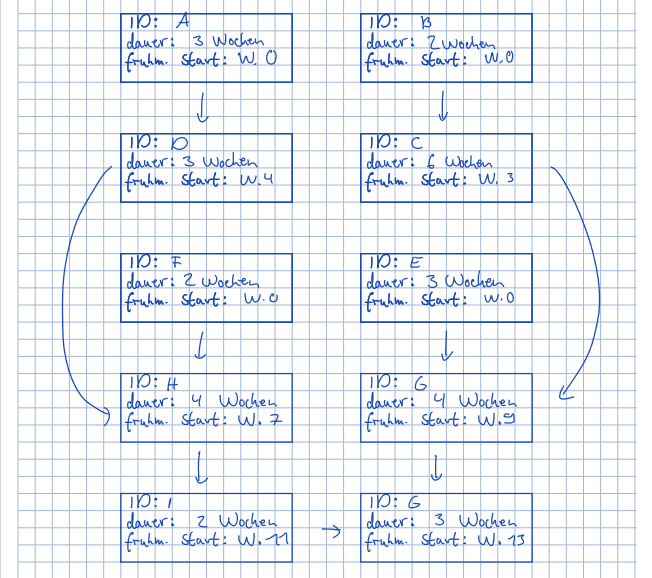
\includegraphics[width=1\textwidth]{src/u12/task3/a.png} 
    
\newpage
    % /////////////////////// b /////////////////////////
    \item {\itshape Erstellen Sie ein Gantt-Chart, das die zeitlichen Abhängigkeiten der Aufgaben sichtbar macht.}
    
    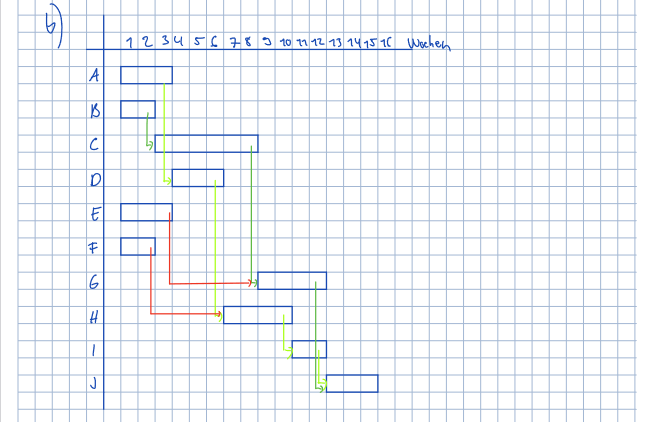
\includegraphics[width=1\textwidth]{src/u12/task3/b.png} 

    % /////////////////////// c /////////////////////////
    \item {\itshape Ermitteln Sie den/die kritischen Pfad/e, die kürzeste Projektlaufzeit, und für alle Aktivitäten jeweils die Pufferzeit (slack time).}
        \begin{itemize}
            \item \textbf{kritische Pfade} aus Aufgabe b) der hell grüne und dunkel grüne Pfad.
            \item \textbf{kürzeste Projektlaufzeit} aus Aufgabe b) ersichtlich: 15 Wochen
            \item[] \begin{tabular}{|l|l|}
                \hline
                \textbf{Aktivitäten} &  \textbf{Pufferzeit (slack time)} in Wochen\\ \hline  
                A & 0 \\ \hline 
                B & 0 \\ \hline 
                C & 2 \\ \hline 
                D & 3 \\ \hline 
                E & 0 \\ \hline 
                F & 0 \\ \hline 
                G & 8 \\ \hline 
                H & 6 \\ \hline 
                I & 10 \\ \hline 
                J & 12\\ \hline 
            \end{tabular}
        \end{itemize}

\newpage
    % /////////////////////// d /////////////////////////
    \item {\itshape Nehmen Sie hypothetisch an, dass Sie den Projektablauf (bei gegebenen Abhängigkeiten) bestmöglich parallelisieren wollen, also die Projektlaufzeit minimieren wollen.Wie hoch wäre der Personalbedarf Pmax, also die größte sinnvolle Teamgröße ab der weitere Personen keine Beschleunigung mehr ergeben? Stellen Sie eine mögliche Aufgabenverteilung für n = Pmax graphisch dar (etwa wie in Abb. 1). Geben Sie für diese Verteilung auch jeweils die Pufferzeiten aller Aufgaben, sowie die Projektlaufzeit an.}
        \begin{itemize}
            \item \textbf{Pmax} = 5 = n
            \item \textbf{Projektlaufzeit}: 15 Wochen
            \item[] \begin{tabular}{|l|l|}
                \hline
                \textbf{Aktivitäten} &  \textbf{Pufferzeit (slack time)} in Wochen\\ \hline  
                A & 0 \\ \hline 
                B & 0 \\ \hline 
                C & 2 \\ \hline 
                D & 3 \\ \hline 
                E & 0 \\ \hline 
                F & 3 (einzige Änderung) \\ \hline 
                G & 8 \\ \hline 
                H & 6 \\ \hline 
                I & 10 \\ \hline 
                J & 12\\ \hline 
            \end{tabular}
            
            \item[] 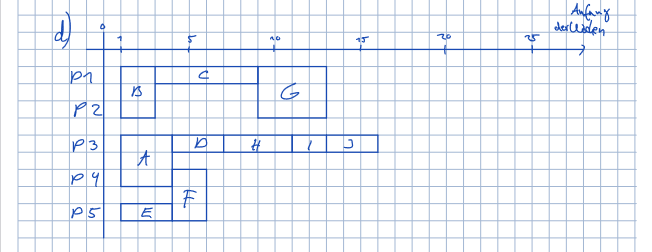
\includegraphics[width=1\textwidth]{src/u12/task3/d.png} 
        \end{itemize}
    
\newpage
    % /////////////////////// e /////////////////////////
    \item {\itshape Nehmen Sie an, Sie könnten nur zwei Entwickler/innen für dieses Projekt abstellen. Was wäre hier die kürzeste Projektlaufzeit? Stellen Sie eine mögliche Aufgabenverteilung für n = 2 graphisch dar. Geben Sie auch für diese Verteilung die Pufferzeiten und die Gesamtlaufzeit an.}
        \begin{itemize}
            \item \textbf{n} = 2
            \item \textbf{Projektlaufzeit}: 26 Wochen
            \item[] \begin{tabular}{|l|l|}
                \hline
                \textbf{Aktivitäten} &  \textbf{Pufferzeit (slack time)} in Wochen\\ \hline  
                A & 0 \\ \hline 
                B & 3 \\ \hline 
                C & 5 \\ \hline 
                D & 3 \\ \hline 
                E & 8 \\ \hline 
                F & 11 \\ \hline 
                G & 13 \\ \hline 
                H & 17 \\ \hline 
                I & 21 \\ \hline 
                J & 23\\ \hline 
            \end{tabular}
            
            \item[] 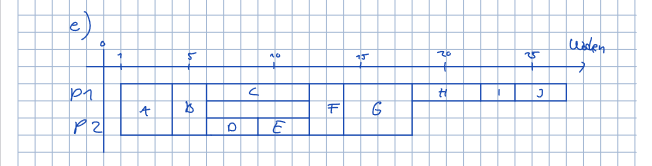
\includegraphics[width=1\textwidth]{src/u12/task3/e.png} 
        \end{itemize}
    
\newpage
    % /////////////////////// f /////////////////////////
    \item {\itshape Stellen Sie Aufgabenverteilungen für alle weiteren möglichen Teamgrößen n (d.h. also 2 < n < Pmax) graphisch dar, sodass jeweils die Projektlaufzeit möglichst kurz ist. Geben Sie wiederum für jede Verteilung die Projektlaufzeit und die Pufferzeiten an.}
        \begin{itemize}
            \item \textbf{n} = 3
            \item \textbf{Projektlaufzeit}: 19 Wochen
            \item[] \begin{tabular}{|l|l|}
                \hline
                \textbf{Aktivitäten} &  \textbf{Pufferzeit (slack time)} in Wochen\\ \hline  
                A & 0 \\ \hline 
                B & 2 \\ \hline 
                C & 9 \\ \hline 
                D & 10 \\ \hline 
                E & 3 \\ \hline 
                F & 7 \\ \hline 
                G & 13 \\ \hline 
                H & 14 \\ \hline 
                I & 16 \\ \hline 
                J & 19 \\ \hline 
            \end{tabular}
            
            \item[] 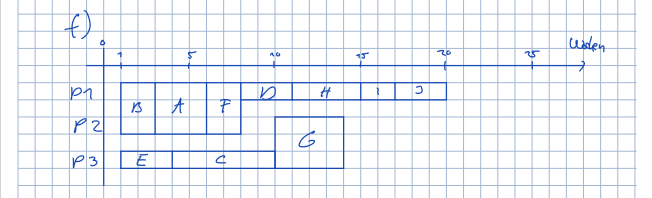
\includegraphics[width=1\textwidth]{src/u12/task3/f_1.png} 
        \end{itemize}
        
        \begin{itemize}
            \item \textbf{n} = 4
            \item \textbf{Projektlaufzeit}: 17 Wochen
            \item[] \begin{tabular}{|l|l|}
                \hline
                \textbf{Aktivitäten} &  \textbf{Pufferzeit (slack time)} in Wochen\\ \hline  
                A & 0 \\ \hline 
                B & 0 \\ \hline 
                C & 2 \\ \hline 
                D & 5 \\ \hline 
                E & 2 \\ \hline 
                F & 3 \\ \hline 
                G & 5 \\ \hline 
                H & 8 \\ \hline 
                I & 12 \\ \hline 
                J & 17 \\ \hline 
            \end{tabular}
            
            \item[] 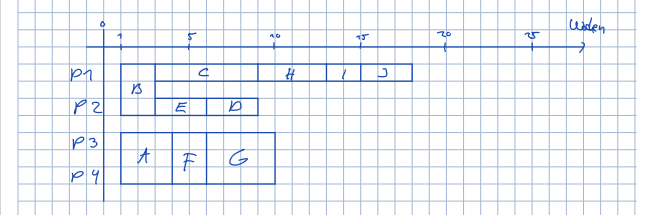
\includegraphics[width=1\textwidth]{src/u12/task3/f_2.png} 
        \end{itemize}
    
    
    % /////////////////////// g /////////////////////////
    \item {\itshape Betrachten Sie Ihre möglichen Projektabläufe (also für alle Teamgrößen von 2 bis einschließlich Pmax) und fällen Sie eine Entscheidung: Wie viele Entwickler/innen setzen Sie nun auf dieses Projekt an? Erläutern Sie Ihre Entscheidung: Vergleichen Sie Ihre Optionen explizit nach mindestens drei Gesichtspunkten.}
    \begin{itemize}
        \item Wir haben folgende Gesichtspunkte mit in Betracht gezogen:
        \begin{enumerate}[1.]
            \item Teamgröße. (Weniger Mitarbeiter -> Weniger Einarbeitung, Kommunikation und Kosten.)
            \item Projektlaufzeit. (Je kürzer desto besser)
            \item slack time. (Auch von Mitarbeitern. Mitarbeiter sollen möglichst immer Arbeit haben)
        \end{enumerate}
        \item Aufgrund der oberen Gesichtspunkte haben wir uns für 3 Mitarbeiter entschieden. Hier finden wir das Verhältnis von Projektlaufzeit (19W) und slack time (der Mitarbeiter (12W)) am besten.
        \item Bei 2 Mitarbeitern wäre uns die Projektlaufzeit zu lang (26W anstatt nur 19W). Und bei 4 Mitarbeitern ist uns der Austausch von mehr slack time zu weniger Projektlaufzeit nicht wert. (Projektlaufzeit verkürzt sich nur um 2 Wochen. Dafür haben die Mitarbeiter nun insgesamt 25 Wochen keine Arbeit nur 12 Wochen)
    \end{itemize}



\end{enumerate}

\end{document}